\documentclass[11pt]{article}

% Compile with: latexmk -xelatex paper.tex
\usepackage{fontspec}
\setmainfont{Latin Modern Roman}
\usepackage{geometry}
\geometry{a4paper, margin=1in}
\usepackage{microtype}
\usepackage{booktabs}
\usepackage{tabularx}
\usepackage{array}
\usepackage{amsmath}
\usepackage{graphicx}
\usepackage{enumitem}
\setlist{nosep, leftmargin=1.4em}
\usepackage{xcolor}
\usepackage[colorlinks=true, linkcolor=black, citecolor=blue!55!black,
            urlcolor=blue!55!black]{hyperref}
\usepackage[backend=biber, style=numeric-comp, sorting=none, url=true,
            doi=false, isbn=false]{biblatex}
\addbibresource{../proposal/references.bib}
\usepackage{titlesec}
\titleformat{\section}{\large\bfseries}{\thesection}{0.6em}{}
\titleformat{\subsection}{\normalsize\bfseries}{\thesubsection}{0.6em}{}
\titlespacing*{\section}{0pt}{1.1em}{0.5em}
\titlespacing*{\subsection}{0pt}{0.8em}{0.35em}
\newcolumntype{Y}{>{\raggedright\arraybackslash}X}
\setlength{\emergencystretch}{3em}

\title{\vspace{-2.2em}\textbf{Defense-Aware Attacks on Content Disarm and Reconstruction
and JPEG as Defenses for a Vision-Language Model}}
\author{Nông Văn Tình}
\date{Advanced Computer Vision (ACV / MCS) \\ \today}

\begin{document}
\maketitle
\vspace{-1.2em}

\begin{abstract}
\noindent
Content Disarm and Reconstruction (CDR) is recommended as a defense against adversarial
images and prompt injection for multimodal models, but the evidence for it comes from
attackers who do not know the defense exists. We attack a vision-language model
(LLaVA-1.5-7B) with a targeted $L_\infty$ attack that is optimized through the defense
(backward pass through a differentiable surrogate, forward pass through the real defense
where it can run) and score every result through the real tool. The defenses are JPEG
quality~50 and Dangerzone, an open-source CDR tool, run with an adapter that does not add
a JPEG stage of its own. On 200 images with a pre-registered analysis of six paired tests,
the defense-aware attack beats the defense-unaware attack in all six. At $16/255$ it
succeeds on 21\% of the images through JPEG~50 and on 76.5\% through Dangerzone, against
0\% and 1.5\% for the unaware attack. At $8/255$ the rates are 9\% and 29\%. Under
defense-aware attack Dangerzone is easier to break than JPEG~50, by 20 points at $8/255$
and 55.5 points at $16/255$. All attacks stopped at 500 steps before their loss had
flattened, so every rate is a lower bound, and the Dangerzone and JPEG attacks are not
guaranteed to be equally strong. The data support the claim that neither defense holds
against an attacker who knows it. They give no support for the claim that CDR protects
better than JPEG. They cover one model, one benign target and one CDR tool.
\end{abstract}

% ======================================================================
\section{Introduction}

A small, bounded change to the pixels of an image can steer what a vision-language model
(VLM) says about it~\cite{qi2024visualaaai}. A common model-agnostic defense is to
re-encode the input before the model sees it~\cite{guo2018countering}. Security practice
adds another candidate: Content Disarm and Reconstruction (CDR) parses a file, keeps only
content it can validate, and rebuilds a clean file. Published guidance already recommends
multimedia CDR against prompt injection in agent pipelines~\cite{safm49}.

Whether CDR defends a model against adversarial pixels is an empirical question, and the
answer depends on the attacker. A defense that works against an attacker who ignores it
often fails once the attacker optimizes through it~\cite{athalye2018obfuscated,tramer2020adaptive}.
In an earlier non-adaptive study with the same model and images, every defense we tried
removed almost all of a targeted attack: of 185 attacks that worked without a defense, none
survived Dangerzone or JPEG~50. That result says little about an attacker who adapts, and it
has a second problem described in Section~\ref{sec:confound}: the Dangerzone adapter we
used embedded a JPEG~75 image, so its result could not be credited to Dangerzone.

This paper reports the defense-aware follow-up. It asks two questions:
\begin{itemize}
\item \textbf{H1.} Does an attacker who optimizes through the defense recover success
that a defense-unaware attacker does not have?
\item \textbf{H2.} Under defense-aware attack, does Dangerzone differ from JPEG~50?
\end{itemize}
Both were registered before any adaptive result existed (Section~\ref{sec:prereg}).
CDR is an existing technique and Dangerzone~\cite{dangerzone} is an existing tool. The
contribution is the measurement: paired, pre-registered, with the real defense in the
scoring path, and with the limits of the attack stated next to the numbers.

% ======================================================================
\section{Setup}

\subsection{Model, data and success criterion}
The model is LLaVA-1.5-7B~\cite{liu2023llava} (\texttt{llava-hf/llava-1.5-7b-hf}) with its
CLIP ViT-L/14-336 vision tower~\cite{radford2021clip}, loaded in 4-bit NF4 with fp16
compute and decoded greedily. The question is ``What is the main object in this image?
Answer with a single lowercase word.''

The 200 images are 10 from each of 20 ImageNet classes~\cite{deng2009imagenet}, resized to
$336\times336$. The set is fixed, and the 20 classes are not a random draw from 1000. Each
image has a benign target label, the next class in sorted order. An attack succeeds when the
model's greedy answer through the defense contains the target word. This measures a
targeted output hijack to an innocuous label. No harmful content is generated.

\subsection{Defenses}
Every number in this paper is scored through the real defense.
\begin{itemize}
\item \textbf{JPEG 90, 75, 50:} Pillow, 4:2:0 subsampling.
\item \textbf{Dangerzone 0.11.0}~\cite{dangerzone}, run through rootless Podman. It works
on documents, so each image is wrapped in a one-page PDF, sanitized, and rasterized back
to $336\times336$. We use the \emph{lossless adapter}, which embeds the image in the PDF as
lossless bytes. The \emph{legacy adapter} uses Pillow's PDF writer, which re-encodes the
image as JPEG~75 first. Section~\ref{sec:confound} explains why the two are kept apart.
\end{itemize}
ICDR~\cite{icdr,openimagecdr} was planned as a second CDR tool. Its committed code depends
on a commercial imaging library and does not compile, so it was not run.

\subsection{Defense-aware attack}
The attack is targeted $L_\infty$ projected gradient descent~\cite{madry2018pgd} with a
sign-gradient step of $1/255$, a random start, seed 1234, and 500 steps. The loss is
teacher-forced cross-entropy toward the target word, computed on the image \emph{after}
the defense. Gradients come from a backward pass through a differentiable surrogate with a
straight-through estimator for rounding (BPDA~\cite{athalye2018obfuscated}). The two
surrogates are:
\begin{itemize}
\item \textbf{JPEG 50.} A differentiable JPEG (blockwise DCT, quantization with the libjpeg
tables, straight-through rounding). The forward pass is the real Pillow codec, so the model
is attacked on exactly the pixels it will see.
\item \textbf{Dangerzone.} The real tool cannot run on the GPU host, so a separable banded
linear map (bandwidth 8) is fitted to the real tool's input and output pairs (600 training and
200 held-out pairs). Its held-out PSNR against the real output is 48.9~dB on clean and
48.1~dB on adversarial inputs. The attack uses the surrogate in both passes. Final success
is always scored through the real tool.
\end{itemize}
The update has no momentum and a constant step, so the iterate is the whole optimizer state
and an interrupted attack resumes exactly. Budgets are $\epsilon\in\{8,16\}/255$. A change of
$16/255$ lets each colour channel move by at most 16 of 255 levels, about 6\%.

\subsection{Non-adaptive baseline}
The defense-unaware condition is the stored attack from the earlier study: PGD against the
undefended model, 200 steps of $1/255$, same images, targets and seed, scored through each
real defense. The stored arrays were rescored in a control run (\texttt{controls\_v1}), which
is the baseline here. Without a defense this attack reaches 10.5\%, 26.5\% and 56\% of the
images at $4$, $8$ and $16/255$ (21, 53 and 112 of 200).

\subsection{The adapter confound}
\label{sec:confound}
The legacy Dangerzone adapter produces a JPEG~75 image, then a 150~dpi raster, then
Dangerzone's own conversion. The embedded image is bit-identical to Pillow's JPEG~75
output. JPEG~75 alone defeated 184 of the 185 attacks that worked undefended, so the earlier
Dangerzone result could not be attributed to Dangerzone. The lossless adapter was added
for this study. The two adapters are separate conditions in every table, and no number
pools them. Clean-image preservation is similar for both: the model's own clean answer is
unchanged on 93.5\% of images through the lossless adapter and 91.5\% through the legacy one
(JPEG~50: 92\%).

\subsection{Pre-registration, tests and statistics}
\label{sec:prereg}
The analysis was registered in the repository before any adaptive result existed
(files \texttt{phase2\_preregistration.md} and \texttt{analysis\_plan.yaml}). It is an
internal registration timestamped by the commit history, not an external registry entry.
The confirmatory family has six tests: H1 for JPEG~50 and for Dangerzone, and H2, each at
$8/255$ and $16/255$. Each test pairs the same 200 images across two attack conditions.
We report exact McNemar tests on the discordant pairs, Clopper--Pearson intervals for rates,
Newcombe intervals for paired differences, and Holm correction over the six tests at
$\alpha=0.05$. The minimum effect of interest is 15 points. At $N=200$ and a discordant rate
of 0.3 the simulated power to detect a 15-point difference is 0.89, and differences below
about 10 points cannot be resolved. A 50-image screen preceded the confirmatory runs. It was
exploratory, and the four confirmatory conditions were chosen after it (Appendix~\ref{app:dev}).

\subsection{Compute}
The attacks take 12 to 15 minutes per image on a Colab T4, about 180 GPU hours for the four
confirmatory runs. State lived on Drive, and each session resumed from the stored iterate.
Sanitizing ran on a local machine with rootless Podman. GPU runs are not bit-reproducible.

% ======================================================================
\section{Results}

\subsection{H1: knowing the defense recovers success}
Table~\ref{tab:h1} and Figure~\ref{fig:asr} give the targeted success rates. All four
adaptive differences are significant after Holm correction, and in every case the discordant
pairs run in one direction only: 42 images flip to success through JPEG~50 and none flip
the other way at $16/255$, and 150 against 0 through Dangerzone.

\begin{table}[t]
\centering
\caption{Targeted success through the real defense, $N=200$ per cell. Rates have exact 95\%
intervals. The difference is adaptive minus non-adaptive with a Newcombe interval. $b/c$ are
the discordant pairs (success only under the adaptive attack / only under the non-adaptive
attack). $p_{\mathrm{Holm}}$ is over the six registered tests.}
\label{tab:h1}
\footnotesize
\setlength{\tabcolsep}{3.5pt}
\begin{tabular}{llccccc}
\toprule
Defense & $\epsilon$ & Non-adaptive & Adaptive & Diff. (pts) & $b/c$ & $p_{\mathrm{Holm}}$ \\
\midrule
JPEG 50    & 8/255  & 0/200 (0\%)    & 18/200 (9\%)    & 9.0 [5.3, 13.8]   & 18/0   & $8\times10^{-6}$ \\
Dangerzone & 8/255  & 1/200 (0.5\%)  & 58/200 (29\%)   & 28.5 [22.5, 35.1] & 57/0   & $6\times10^{-17}$ \\
JPEG 50    & 16/255 & 0/200 (0\%)    & 42/200 (21\%)   & 21.0 [15.6, 27.2] & 42/0   & $1\times10^{-12}$ \\
Dangerzone & 16/255 & 3/200 (1.5\%)  & 153/200 (76.5\%) & 75.0 [68.2, 80.4] & 150/0  & $8\times10^{-45}$ \\
\bottomrule
\end{tabular}
\end{table}

\begin{figure}[t]
\centering
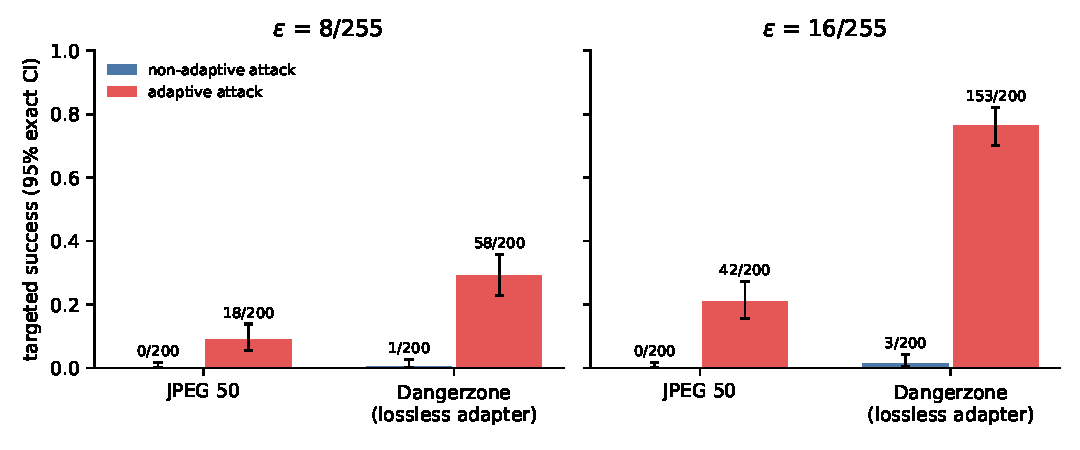
\includegraphics[width=0.92\linewidth]{figures/fig_confirmatory_asr.pdf}
\caption{Targeted success through the real defense for the non-adaptive and the adaptive
attack (error bars: exact 95\% intervals; counts above the bars).}
\label{fig:asr}
\end{figure}

The JPEG~50 effect at $8/255$ is the smallest, 9 points with an interval of 5 to 14. Its
interval lies below the 15-point minimum effect of interest, so it is a detected effect that
is smaller than the one the study was powered to resolve.

\subsection{H2: Dangerzone against JPEG 50 under defense-aware attack}
With each defense attacked through its own surrogate for the same 500 steps, the success rate
is higher against Dangerzone than against JPEG~50: 29\% against 9\% at $8/255$ (difference
20 points, interval 14 to 26, 43 discordant pairs against 3) and 76.5\% against 21\% at
$16/255$ (55.5 points, interval 48 to 62, 113 against 2). Both are significant after
correction, and both intervals exclude the 15-point effect. Figure~\ref{fig:diff} shows all
six differences.

\begin{figure}[t]
\centering
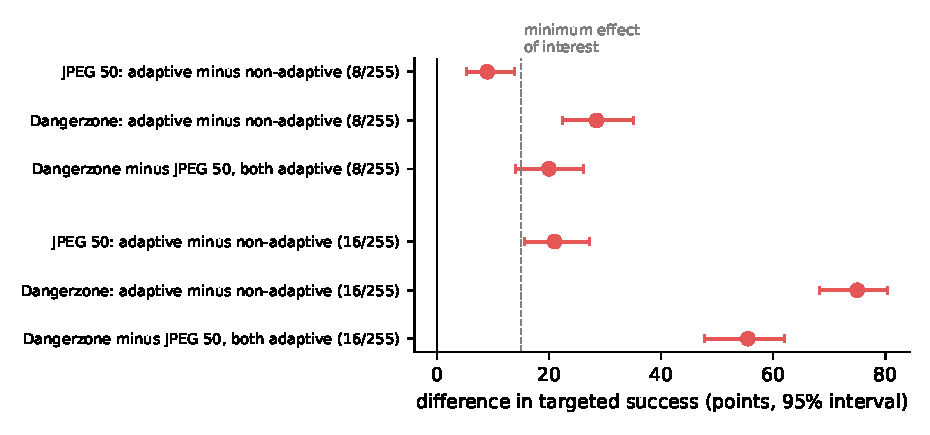
\includegraphics[width=0.85\linewidth]{figures/fig_paired_differences.pdf}
\caption{The six registered paired differences with 95\% intervals. The dashed line is the
15-point minimum effect of interest.}
\label{fig:diff}
\end{figure}

This is a comparison of two attacks as well as two defenses, and it should not be read as a
ranking of the defenses (Section~\ref{sec:limits}).

\subsection{The adaptive images are specific to their defense}
Scored through other defenses, the images optimized through Dangerzone almost never succeed:
at $16/255$ they reach 1, 0 and 0 of 200 through JPEG 90, 75 and 50 (16 of 200 undefended).
The images optimized through JPEG~50 do not carry over to its neighbours either: at $16/255$
they succeed on 12 and 10 of 200 through JPEG 90 and 75, about the 11 they reach undefended,
and 42 through JPEG~50. At $8/255$ the counts are 12 and 3, against 18 through JPEG~50. The
attack therefore exploits the specific defense it was given, and an attacker who wants
success through a deployed defense has to attack that one.

\subsection{Optimization and validity gates}
Figure~\ref{fig:loss} shows the median target loss during the attack. The defended loss
(measured on the real defense after the attack) is lower for the adaptive image than for the
non-adaptive image on 200 of 200 images in every run (medians 0.43 against 5.0 for Dangerzone
at $16/255$, 1.63 against 5.7 at $8/255$; 2.70 against 7.5 and 4.46 against 7.7 for JPEG~50).
Every run passed the gates registered before the study: all jobs finished, the perturbation
stayed inside the ball, and no real-defense evaluation failed. The Dangerzone surrogate meets
the 40~dB fidelity threshold.

None of the attacks converged. The median loss still fell by 17.7\% and 13.6\% over the last
100 steps, relative to the 100 before them, of the Dangerzone runs ($16$ and $8/255$) and by 7.8\% and 1.9\% for JPEG~50. The
JPEG~50 attack ends at a loss of 2.7 to 4.5, well above the 0.4 to 1.6 that the Dangerzone
attack reaches, so it is farther from success at the same step count. In a pilot on ten images
at $16/255$, the JPEG~50 success rate rose with steps (0/10 at 200, 4/10 at 500, 6/10 at
1000, 7/10 at 2000). Every rate in Table~\ref{tab:h1} is therefore at or below what a longer
attack would give.

\begin{figure}[t]
\centering
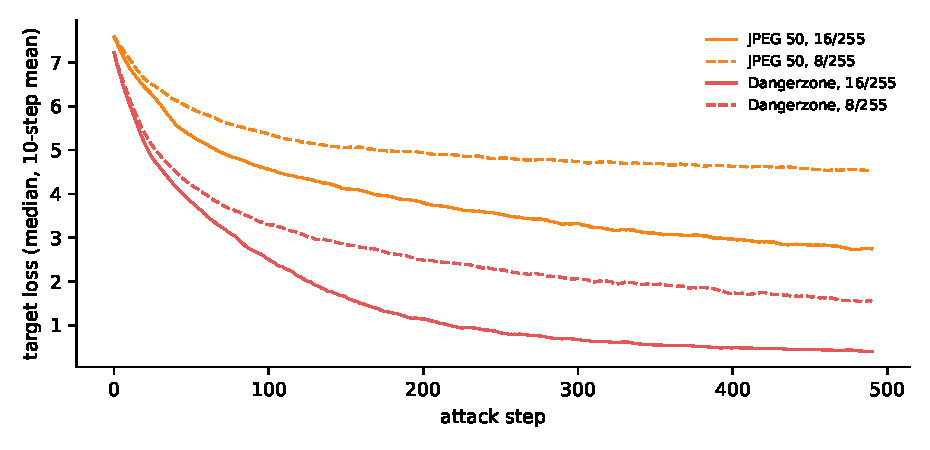
\includegraphics[width=0.8\linewidth]{figures/fig_loss_curves.pdf}
\caption{Median target loss during the 500-step attack (10-step mean). Dangerzone curves use
the surrogate forward pass, JPEG curves the real codec.}
\label{fig:loss}
\end{figure}

\subsection{Exploratory screen: the legacy adapter}
A 50-image screen preceded the confirmatory runs and included the legacy adapter, which was
not repeated at $N=200$. At $16/255$ the success rate through real Dangerzone was 42\% with
the legacy adapter and 80\% with the lossless adapter (JPEG~50: 24\%). At $8/255$ the rates
were 14\%, 26\% and 12\%. These are exploratory, with Holm correction inside the screen's own
family. The legacy adapter was harder to attack than the lossless one. Its extra JPEG~75
stage is the likely reason, which would make the difference an effect of JPEG and not of CDR,
but we did not test this directly.

% ======================================================================
\section{Discussion}

An attacker who knows the defense gets large gains against both tools. Against Dangerzone
with the lossless adapter the gain is 75 points at $16/255$, and JPEG~50 is also broken on
21\% of the images at the same budget. The earlier result that every defense removes almost
all of the attack describes an attacker who ignores the defense. It should not be cited as a
statement about robustness.

Dangerzone's sanitization removes what a defense-unaware perturbation depends on, and
JPEG~50 does too. Neither removes the information an attacker needs once the defense is in
the optimization loop. The lossless Dangerzone pipeline is close to a resampling and a
re-rasterization, which are smooth and nearly invertible at the scale of the perturbation, so
gradients pass through them well. JPEG~50 quantizes in the DCT domain, which discards more
information, and the attack makes less progress through it. We did not run an experiment
that isolates this explanation, and it should be treated as a hypothesis.

The data do not support a claim that CDR protects better than JPEG, in either direction. The
H2 result favours JPEG~50 at equal steps, but the JPEG attack stops at a higher loss and both
surrogates differ in kind (real forward for JPEG, fitted forward for Dangerzone). A
converged attack on JPEG~50 could erase the gap or reverse it.

% ======================================================================
\section{Limitations}
\label{sec:limits}

\begin{itemize}
\item \textbf{Unconverged attacks.} All rates are lower bounds. A zero under these attacks
would not have shown robustness, and the nonzero rates understate what a longer attack gets.
\item \textbf{Step budgets differ between the two attack conditions.} The adaptive attack
runs 500 steps and the stored non-adaptive attack 200. We did not run a 500-step
non-adaptive control, so H1 combines knowledge of the defense with a larger step budget, and
we cannot say how much of each gain comes from the extra steps. The size of the gains and the
pilot's rise with steps both suggest that knowledge of the defense is the larger part, but
this is a judgment and not a measurement.
\item \textbf{Unequal attack strength across defenses.} JPEG~50 is attacked through the real
codec and a straight-through gradient, Dangerzone through a fitted linear surrogate. H2
compares both the defenses and the attacks.
\item \textbf{One model, one target rule, 20 classes, one CDR tool.} We did not run a second
VLM, a typographic or prompt-injection attack, ICDR, MetaDefender Core or other CDR products,
or $4/255$ in the adaptive setting. Results do not carry over to those cases.
\item \textbf{The surrogate is an approximation.} Its 48 to 49~dB fidelity is high, and
success is scored on the real tool, but the attack direction is only as good as the
surrogate's Jacobian.
\item \textbf{One seed and a stored baseline.} GPU runs are not bit-reproducible. Thirty-nine
of the 600 non-adaptive rows in the original run used pixels different from the stored
arrays. This changes the undefended count by one image and none of the defended counts
(Appendix~\ref{app:dev}). The baseline here comes from the rescored stored arrays.
\item \textbf{The registration is internal.} It is timestamped by the commit history and was
never filed with an external registry.
\end{itemize}

% ======================================================================
\section{Conclusion}

Against an attacker who optimizes through the defense, both JPEG~50 and Dangerzone fail on a
substantial share of 200 images at $16/255$ (21\% and 76.5\%) and a smaller share at $8/255$
(9\% and 29\%), where the defense-unaware attack reached 0\% and 0.5\%. The study supports
the statement that defenses evaluated against defense-unaware attacks should not be called
robust, and it does not support a ranking of CDR against JPEG. Closing the gaps listed above,
starting with a longer attack and a 500-step non-adaptive control, is the direct next step.

\section*{Reproducibility}
\begin{sloppypar}
Code, configurations, the registration and the analysis scripts are in the project
repository. The pre-registered analysis is \texttt{scripts/analyze\_confirmatory.py}
under \texttt{configs/analysis\_plan.yaml}, and the figures come from
\texttt{scripts/make\_paper\_figures.py}. The four confirmatory runs are
\texttt{conf\_jpeg50\_e08}, \texttt{conf\_jpeg50\_e16}, \texttt{conf\_dz\_ll\_e08} and
\texttt{conf\_dz\_ll\_e16}, with the non-adaptive baseline in \texttt{controls\_v1}. The
non-adaptive baseline tag is \texttt{baseline-nonadaptive-v1}. The model weights and the
ImageNet images come from their public sources.
\end{sloppypar}

\appendix
\section{Deviations from the registration}
\label{app:dev}

\begin{itemize}
\item The registered baseline-reproduction gate G5 (at least 99\% raw-answer agreement
between the rescored controls and the original run) failed at 96.8\% (581 of 600) and is
reported as failed. The 19 differing answers all came from the 39 rows whose input pixels
differed between the two runs, most likely because those attacks were crafted again after
the first evaluation. Two diagnostic gates, G5a and G5b, were added after seeing this. Both
restrict to identical inputs and pass (561 of 561). The undefended count changes by one
image; the JPEG results are identical in both runs. The earlier report needs an erratum, and
its conclusions do not change.
\item The registered JPEG~50 extension schedule was changed from 400 to 500, 1000 and 2000
steps after the 200-step pilot loss was still falling.
\item The screen images were stratified over the 20 classes instead of taking the first 50 in
manifest order, which would have covered only 5 classes. $4/255$ was left out of the adaptive
runs for compute reasons.
\item The confirmatory step budget was set to 500 for all adaptive attacks, a compute cap
chosen after the screen, so the attacks are at equal steps but unconverged.
\item The confirmatory conditions (JPEG~50 and lossless Dangerzone at two budgets) were chosen
after the screen. The legacy adapter was not run at $N=200$.
\end{itemize}

\printbibliography

\end{document}
